\documentclass{standalone}
\usepackage{tikz}
\usetikzlibrary{patterns, positioning}
\usepackage[sfdefault]{ClearSans} %% option 'sfdefault' activates Clear Sans as the default text font
\usepackage[T1]{fontenc}

\begin{document}
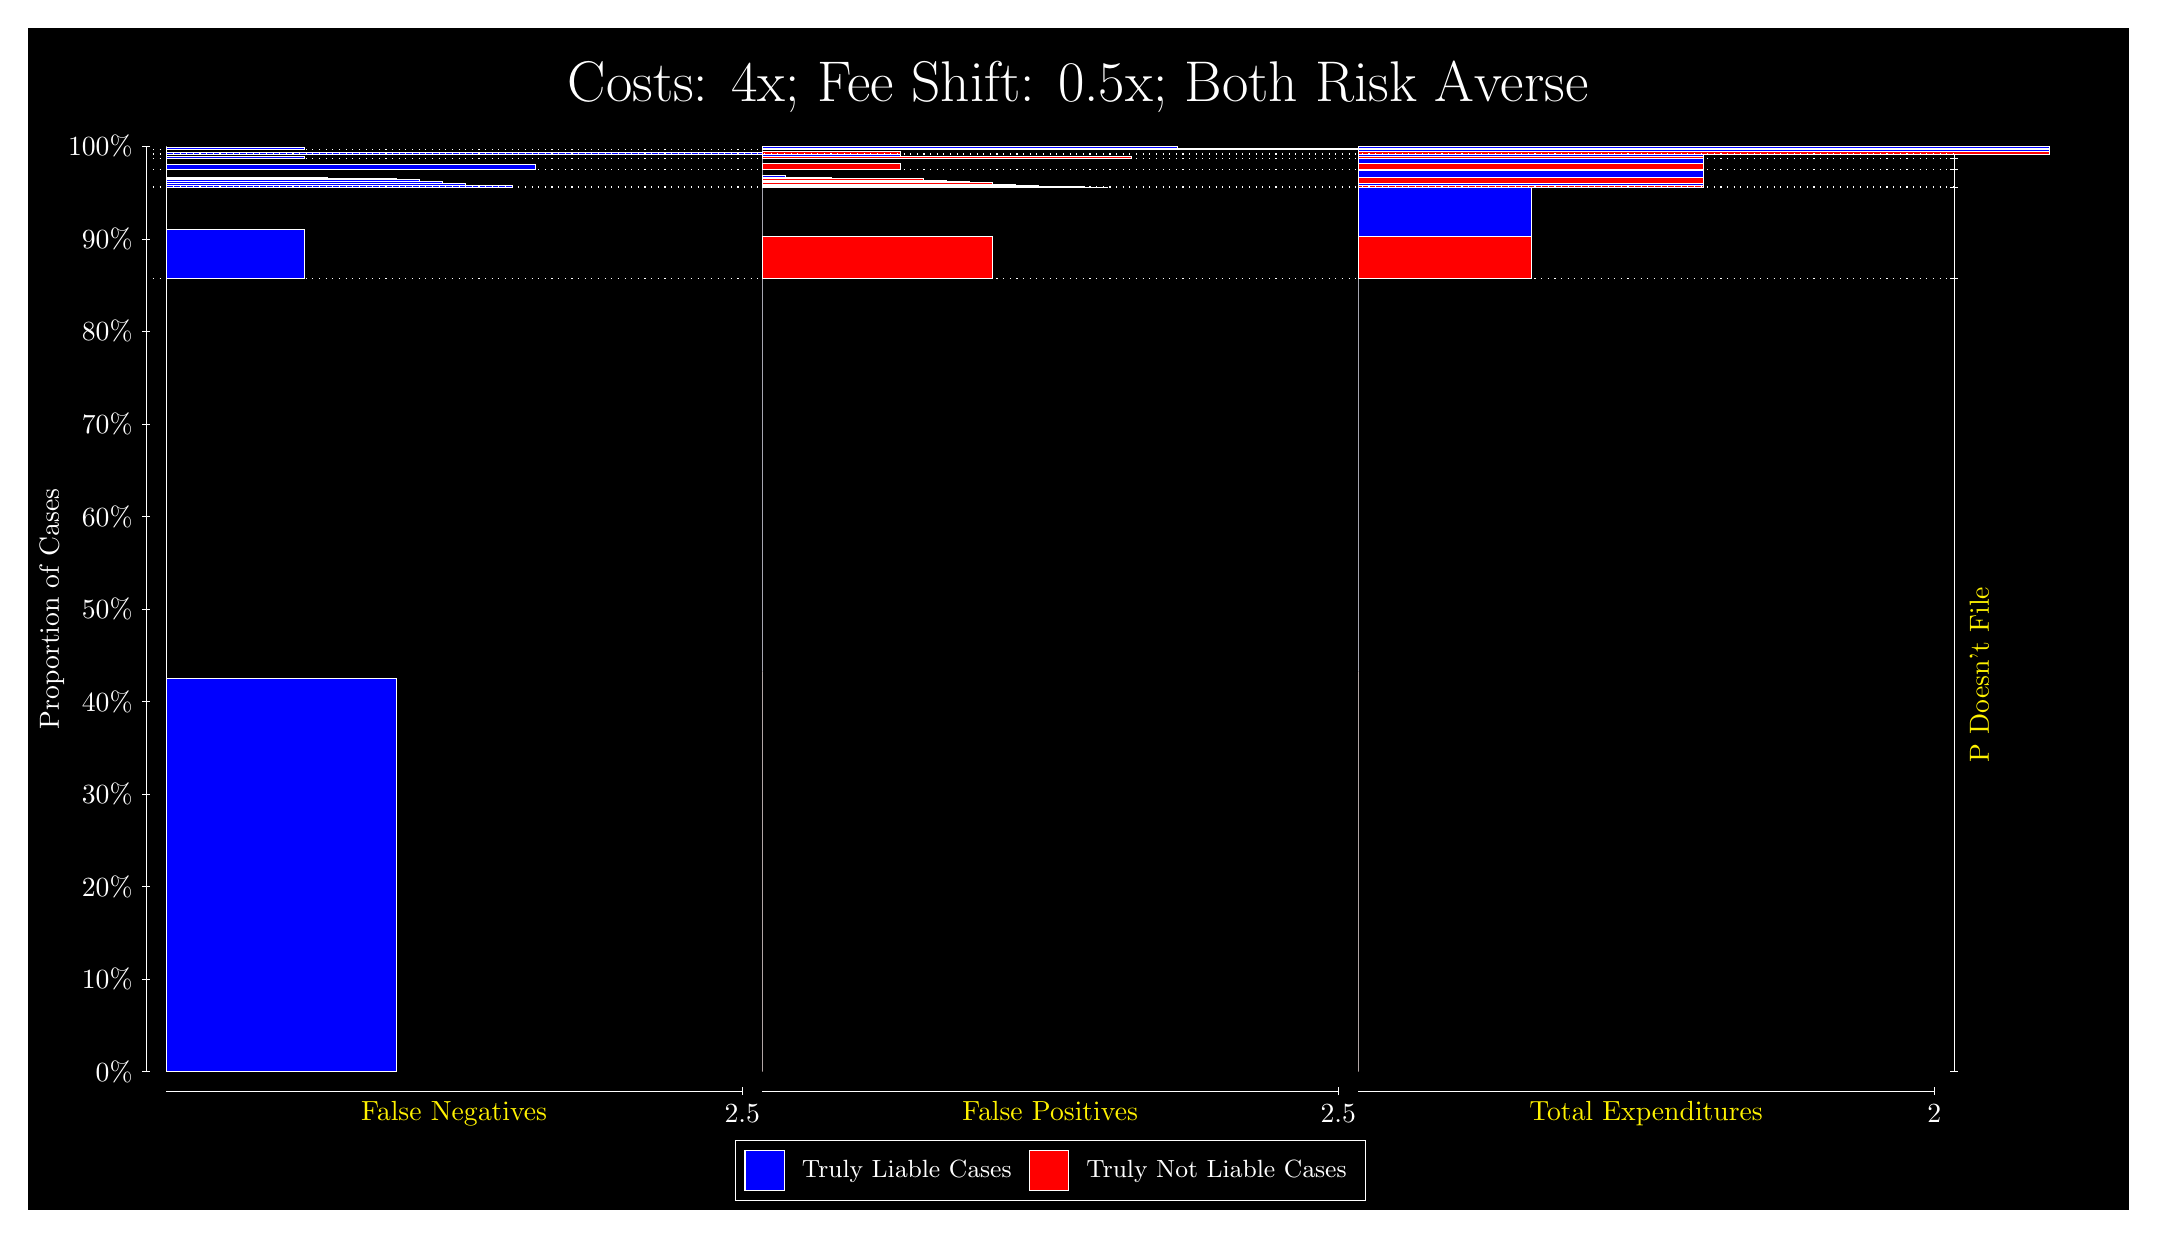
\begin{tikzpicture}
\draw[fill=black] (0,0) rectangle (26.667,15);
\draw[text=white] (0,13.5) rectangle (26.667,15) node[midway] {\huge Costs: 4x; Fee Shift: 0.5x; Both Risk Averse};
\draw[white, very thin] (1.5,1.75) -- (1.5,13.5);
\node[rotate=90, text=white, anchor=center] at (0.3, 7.625) {Proportion of Cases};
\draw[white, very thin] (1.45,1.75) -- (1.55,1.75);
\node[text=white, anchor=east] at (1.45, 1.75) {0\%};
\draw[white, very thin] (1.45,2.925) -- (1.55,2.925);
\node[text=white, anchor=east] at (1.45, 2.925) {10\%};
\draw[white, very thin] (1.45,4.1) -- (1.55,4.1);
\node[text=white, anchor=east] at (1.45, 4.1) {20\%};
\draw[white, very thin] (1.45,5.275) -- (1.55,5.275);
\node[text=white, anchor=east] at (1.45, 5.275) {30\%};
\draw[white, very thin] (1.45,6.45) -- (1.55,6.45);
\node[text=white, anchor=east] at (1.45, 6.45) {40\%};
\draw[white, very thin] (1.45,7.625) -- (1.55,7.625);
\node[text=white, anchor=east] at (1.45, 7.625) {50\%};
\draw[white, very thin] (1.45,8.8) -- (1.55,8.8);
\node[text=white, anchor=east] at (1.45, 8.8) {60\%};
\draw[white, very thin] (1.45,9.975) -- (1.55,9.975);
\node[text=white, anchor=east] at (1.45, 9.975) {70\%};
\draw[white, very thin] (1.45,11.15) -- (1.55,11.15);
\node[text=white, anchor=east] at (1.45, 11.15) {80\%};
\draw[white, very thin] (1.45,12.325) -- (1.55,12.325);
\node[text=white, anchor=east] at (1.45, 12.325) {90\%};
\draw[white, very thin] (1.45,13.5) -- (1.55,13.5);
\node[text=white, anchor=east] at (1.45, 13.5) {100\%};

\draw[white, very thin] (24.457,1.75) -- (24.457,13.5);
\draw[white, very thin] (24.407,1.75) -- (24.507,1.75);
\node[anchor=west] at (24.407, 1.75) {};
\draw[white, very thin] (24.407,11.825) -- (24.507,11.825);
\node[anchor=west] at (24.407, 11.825) {};
\draw[white, very thin] (24.407,12.983) -- (24.507,12.983);
\node[anchor=west] at (24.407, 12.983) {};
\draw[white, very thin] (24.407,13.209) -- (24.507,13.209);
\node[anchor=west] at (24.407, 13.209) {};
\draw[white, very thin] (24.407,13.342) -- (24.507,13.342);
\node[anchor=west] at (24.407, 13.342) {};
\draw[white, very thin] (24.407,13.402) -- (24.507,13.402);
\node[anchor=west] at (24.407, 13.402) {};
\draw[white, very thin] (24.407,13.458) -- (24.507,13.458);
\node[anchor=west] at (24.407, 13.458) {};
\draw[white, very thin] (24.407,13.5) -- (24.507,13.5);
\node[anchor=west] at (24.407, 13.5) {};

\draw[white, very thin, fill=blue] (1.75,1.75) rectangle (4.6775,6.7425);
\draw[white, very thin, fill=red] (1.75,6.7425) rectangle (1.75,11.825);
\draw[white, very thin, fill=blue] (1.75,11.825) rectangle (3.5065,12.449);
\draw[white, very thin, fill=red] (1.75,12.449) rectangle (1.75,12.983);
\draw[white, very thin, fill=blue] (1.75,12.983) rectangle (6.1413,13.002);
\draw[white, very thin, fill=blue] (1.75,13.002) rectangle (5.8486,13.009);
\draw[white, very thin, fill=blue] (1.75,13.009) rectangle (5.5558,13.033);
\draw[white, very thin, fill=blue] (1.75,13.033) rectangle (5.2631,13.056);
\draw[white, very thin, fill=blue] (1.75,13.056) rectangle (4.9703,13.082);
\draw[white, very thin, fill=blue] (1.75,13.082) rectangle (4.6775,13.089);
\draw[white, very thin, fill=blue] (1.75,13.089) rectangle (4.3848,13.095);
\draw[white, very thin, fill=blue] (1.75,13.095) rectangle (4.092,13.098);
\draw[white, very thin, fill=blue] (1.75,13.098) rectangle (3.7993,13.101);
\draw[white, very thin, fill=red] (1.75,13.101) rectangle (1.75,13.209);
\draw[white, very thin, fill=blue] (1.75,13.209) rectangle (6.4341,13.271);
\draw[white, very thin, fill=red] (1.75,13.271) rectangle (1.75,13.342);
\draw[white, very thin, fill=blue] (1.75,13.342) rectangle (3.5065,13.375);
\draw[white, very thin, fill=red] (1.75,13.375) rectangle (1.75,13.402);
\draw[white, very thin, fill=blue] (1.75,13.402) rectangle (9.9471,13.423);
\draw[white, very thin, fill=red] (1.75,13.423) rectangle (1.75,13.458);
\draw[white, very thin, fill=blue] (1.75,13.458) rectangle (3.5065,13.483);
\draw[white, very thin, fill=red] (1.75,13.483) rectangle (1.75,13.5);
\draw[white, very thin, fill=red] (9.3189,1.75) rectangle (9.3189,6.8327);
\draw[white, very thin, fill=blue] (9.3189,6.8327) rectangle (9.3189,11.825);
\draw[white, very thin, fill=red] (9.3189,11.825) rectangle (12.246,12.359);
\draw[white, very thin, fill=blue] (9.3189,12.359) rectangle (9.3189,12.983);
\draw[white, very thin, fill=red] (9.3189,12.983) rectangle (13.71,12.986);
\draw[white, very thin, fill=red] (9.3189,12.986) rectangle (13.417,12.989);
\draw[white, very thin, fill=red] (9.3189,12.989) rectangle (13.125,12.994);
\draw[white, very thin, fill=red] (9.3189,12.994) rectangle (12.832,13.001);
\draw[white, very thin, fill=red] (9.3189,13.001) rectangle (12.539,13.021);
\draw[white, very thin, fill=red] (9.3189,13.021) rectangle (12.246,13.04);
\draw[white, very thin, fill=red] (9.3189,13.04) rectangle (11.954,13.062);
\draw[white, very thin, fill=red] (9.3189,13.062) rectangle (11.661,13.07);
\draw[white, very thin, fill=red] (9.3189,13.07) rectangle (11.368,13.092);
\draw[white, very thin, fill=blue] (9.3189,13.092) rectangle (10.783,13.095);
\draw[white, very thin, fill=blue] (9.3189,13.095) rectangle (10.49,13.097);
\draw[white, very thin, fill=blue] (9.3189,13.097) rectangle (10.197,13.104);
\draw[white, very thin, fill=blue] (9.3189,13.104) rectangle (9.9044,13.111);
\draw[white, very thin, fill=blue] (9.3189,13.111) rectangle (9.6116,13.137);
\draw[white, very thin, fill=blue] (9.3189,13.137) rectangle (9.3189,13.209);
\draw[white, very thin, fill=red] (9.3189,13.209) rectangle (11.075,13.281);
\draw[white, very thin, fill=blue] (9.3189,13.281) rectangle (9.3189,13.342);
\draw[white, very thin, fill=red] (9.3189,13.342) rectangle (14.003,13.369);
\draw[white, very thin, fill=blue] (9.3189,13.369) rectangle (11.075,13.402);
\draw[white, very thin, fill=red] (9.3189,13.402) rectangle (11.075,13.437);
\draw[white, very thin, fill=blue] (9.3189,13.437) rectangle (9.3189,13.458);
\draw[white, very thin, fill=red] (9.3189,13.458) rectangle (17.516,13.474);
\draw[white, very thin, fill=blue] (9.3189,13.474) rectangle (14.588,13.5);
\draw[white, very thin, fill=red] (16.888,1.75) rectangle (16.888,6.8327);
\draw[white, very thin, fill=blue] (16.888,6.8327) rectangle (16.888,11.825);
\draw[white, very thin, fill=red] (16.888,11.825) rectangle (19.083,12.359);
\draw[white, very thin, fill=blue] (16.888,12.359) rectangle (19.083,12.983);
\draw[white, very thin, fill=red] (16.888,12.983) rectangle (21.279,13.004);
\draw[white, very thin, fill=blue] (16.888,13.004) rectangle (21.279,13.03);
\draw[white, very thin, fill=red] (16.888,13.03) rectangle (21.279,13.109);
\draw[white, very thin, fill=blue] (16.888,13.109) rectangle (21.279,13.192);
\draw[white, very thin, fill=red] (16.888,13.192) rectangle (21.279,13.2);
\draw[white, very thin, fill=blue] (16.888,13.2) rectangle (21.279,13.209);
\draw[white, very thin, fill=red] (16.888,13.209) rectangle (21.279,13.281);
\draw[white, very thin, fill=blue] (16.888,13.281) rectangle (21.279,13.342);
\draw[white, very thin, fill=red] (16.888,13.342) rectangle (21.279,13.369);
\draw[white, very thin, fill=blue] (16.888,13.369) rectangle (21.279,13.402);
\draw[white, very thin, fill=red] (16.888,13.402) rectangle (25.67,13.437);
\draw[white, very thin, fill=blue] (16.888,13.437) rectangle (25.67,13.458);
\draw[white, very thin, fill=red] (16.888,13.458) rectangle (25.67,13.474);
\draw[white, very thin, fill=blue] (16.888,13.474) rectangle (25.67,13.5);
\draw[white, dotted] (1.5,11.825) -- (24.457,11.825);
\draw[white, dotted] (1.5,12.983) -- (24.457,12.983);
\draw[white, dotted] (1.5,13.209) -- (24.457,13.209);
\draw[white, dotted] (1.5,13.342) -- (24.457,13.342);
\draw[white, dotted] (1.5,13.402) -- (24.457,13.402);
\draw[white, dotted] (1.5,13.458) -- (24.457,13.458);
\draw[white, very thin] (1.75,1.5) -- (9.0689,1.5);
\node[text=yellow, anchor=north] at (5.4094, 1.5) {False Negatives};
\draw[white, very thin] (9.0689,1.45) -- (9.0689,1.55);
\node[text=white, anchor=north] at (9.0689, 1.45) {2.5};

\draw[white, very thin] (9.3189,1.5) -- (16.638,1.5);
\node[text=yellow, anchor=north] at (12.978, 1.5) {False Positives};
\draw[white, very thin] (16.638,1.45) -- (16.638,1.55);
\node[text=white, anchor=north] at (16.638, 1.45) {2.5};

\draw[white, very thin] (16.888,1.5) -- (24.207,1.5);
\node[text=yellow, anchor=north] at (20.547, 1.5) {Total Expenditures};
\draw[white, very thin] (24.207,1.45) -- (24.207,1.55);
\node[text=white, anchor=north] at (24.207, 1.45) {2};

\node[text=yellow, centered, rotate=90] at (24.777, 6.7876) {P Doesn't File};







\draw (12.978300999999998,1.5) node[draw=none] (baseCoordinate) {};
\begin{scope}[align=center]
        \matrix[scale=0.5, draw=white, below=0.5cm of baseCoordinate, nodes={draw}, column sep=0.1cm]{
            \node[rectangle, draw, minimum width=0.5cm, minimum height=0.5cm, fill=blue] {}; &
            \node[draw=none, font=\small, text=white] (B) {Truly Liable Cases}; &
            \node[rectangle, draw, minimum width=0.5cm, minimum height=0.5cm, fill=red] {}; &
            \node[draw=none, font=\small, text=white] (B) {Truly Not Liable Cases}; \\
            };
\end{scope}

\end{tikzpicture}
\end{document}